\documentclass[12pt]{article}

\usepackage[margin=1in]{geometry}
\usepackage{times} %should use 12 pt Times New Roman font.
\usepackage[T1]{fontenc}
\usepackage{mathptmx}
\usepackage{hyperref}
\usepackage{url}
\usepackage{microtype}
\usepackage{tikz}
\usetikzlibrary{positioning, shapes}
\usetikzlibrary{decorations.pathmorphing}

\usepackage[style=numeric]{biblatex}
\addbibresource{references.bib}

\usepackage{titlesec}
\titleformat*{\section}{\normalsize\bfseries}
\titleformat*{\subsection}{\normalsize\bfseries}


\begin{document}

\begin{center}
  \textbf{MOOCulus: Iteratively Improving Calculus Instruction}
\end{center}

% PROPOSAL FORMAT
% 
% 1. Proposal overview
% 2. Literature and existing research that informs their proposal
% 3. Context of research (MOOC taught, designed, university/organizational affiliation, MOOC provider, publisher)
% 4. Research questions to be addressed by the project
% 5. Data sources being considered for the project
% 6. Methodology planned for research activities

\section{Proposal overview}

In January 2013, The Ohio State University Mathematics Department
launched its first massive open online course designed to cover the
same content as the local, in-person sections of calculus one.  Part
of this MOOC consisted of a home-built platform designed to deliver
randomly-generated interactive problems to students.  This home-built
adaptive learning platform is usable for much more than calculus: this
same platform has already been re-used for a English writing course
called WexMOOC \parencite{gates-foundation-grant}, and the American
Languages Program at The Ohio State has also reached out to modify the
adaptive learning platform to teach English grammar for their ESL
students.

With tens of thousands of students enrolled in the calculus MOOC,
there have been millions of attempts on homework exercises, with data
on each of these attempts.  Funding is sought to use this data to both
evaluate the success of and improve upon the adaptive learning
platform built at OSU.

\section{Literature}

Calculus is the gateway to science, technology, engineering,
mathematics (STEM) majors; unfortunately, students abandon STEM majors
because of low quality of instruction ``with calculus often cited as a
primary reason'' \parencite{calculus-programs}.  Research universities
are ``doing the worst job in maintaining student confidence in their
mathematical abilities, enjoyment of mathematics, and interest in
continuing with the mathematics that is needed to pursue their
intended careers'' \parencite{calculus-students}.  MOOCs---already
being used at some of the most prestigious US research
universities \parencite{morris2013moocs}---may provide a method by
which research universities can rein in costs and improve student
outcomes \parencite{bowen2013higher}.  In particular, there is
evidence that online assessment techniques can improve student
outcomes in math courses \parencite{angus2009does}.

\subsection{A platform for more than calculus}

For MOOCs to succeed, there must be ``customizable, sustainable
platforms'' \parencite{bowen2013higher} for online instruction;
MOOCulus, a home-built platform from The Ohio State University, is
such a platform for calculus instruction \parencite{evans}, but
MOOCulus has also been used for English courses as
well \parencite{gates-foundation-grant}.  Indeed, discipline-based
education research is inherently interdisciplinary \cite{dber-report};
in studying how best to teach calculus, there are huge opportunities
to think outside the traditional boundaries of the mathematics
department, and to apply the interdisciplinary toolkit of educational
data mining (EDM).  Educational data mining is a relatively recent
development, emerging out of a handful of workshops from the early
00s; since 2008, there has been an annual EDM conference organized by
the International Working Group on Educational Data
Mining \parencite{WIDM:WIDM1075}.

\subsection{Deciding which student interactions should be logged}

Before launching a research project like MOOCulus---or any EDM
project---there is a serious choice to be made: exactly what data will
be mined?  What sorts of data will be stored on each student
interaction?  Some systems have chosen to record the date and time the
student has engaged with various educational
applications \parencite{RomeroZaldivar20121058}; others are looking at
clickstream data \parencite{boyer2013student}.  Going forward, it is
worth considering a format for heterogenous data logging for student
interaction, like the Tin Cap API \parencite{tin-can-api}.

\subsection{Bayesian models}

Much work has been done on using adaptive learning systems to teach
college mathematics, such as ALEKS \parencite{hagerty2005using}, but
they can be difficult for instructors to use.  Some of these use
Bayesian networks to estimate a student's current
understanding \parencite{romero2010educational}.  Hidden Markov models
have also been used in educational data mining for clustering
\parencite{shihdiscovery}.  Such ``machine learning'' techniques can
predict student grades based on only a few
assignments \parencite{predict-grades}, even with incomplete
data \parencite{Zafra201115020}, which make them especially useful for
an adaptive learning platform where not too much student data may be
available on which to base initial predictions.

\subsection{The parameter problem}

A serious issue with all these adaptive learning systems is that
instructors often ``have to provide appropriate values for the
parameters in advance in order to obtain good results/model and
therefore, the user must possess a certain amount of expertise in
order to find the right settings.'' \parencite{romero2010educational}.
Determining appropriate values for these parameters is one of the
major research questions this proposed project addresses.  Some work
has been done in this direction already. There are Java tools for
analyzing Moodle data which attempt to make educational data mining a
bit easier for the novice \parencite{java-data-mining}. However,
currently no easy-to-use version of the Baum-Welch algorithm for EDM
is available to handle the training of a hidden Markov model.

\subsection{Empowering instructors with data analysis}

To verify that such adaptive methods are working, instructors need
easy methods to visualize student data.  David Bressoud---the
researcher behind the largest survey ever of calculus students---asks
the following \parencite{bressoud-sky-falling}:
\begin{quote}
  How can we modify our courses so as to capitalize on the strengths
  and correct the weaknesses that these students bring?  The answers
  to these questions will necessarily be local, highly dependent on
  the nature of a given college or university.
\end{quote}
The Ohio State University (OSU) Department of Mathematics has already
begun to look at these local, contextualized issues.  A pilot study of
``technology enhanced lectures'' at OSU showed significant improvement
in student opinion of the OSU Department of Mathematics, from 29\% of
students having a favorable opinion, to 80\% of students in the
technology-enhanced sections having a favorable opinion
\cite{miller-tech-enhanced-calculus}.  Such affective data can be an
even more important predictor than grades when considering STEM
retention: after all, 81\% of the ``switchers'' who left STEM
nevertheless received a grade of C or higher in their calculus course
\cite{calculus-programs}.


\section{Context of research}

\paragraph{Coursera and MOOCulus.} 
Coursera was chosen as the MOOC provider; some assessments, like the
weekly quizzes, are done entirely within Coursera's platform, but
there are some limitations.  Most seriously, Coursera lacked an easy
method for producing randomly generated math problems, and so the team
at The Ohio State built their own MOOC platform to complement the
missing aspects of Coursera's assessment offerings.  This home-built
MOOC platform is called MOOCulus, and can be explored at
\[
\href{https://mooculus.osu.edu/}{\texttt{https://mooculus.osu.edu/}}
\]
using either a Coursera or Google login.  The platform is a Rails app
which uses Khan Academy's exercise framework \parencite{khan-academy}
for generating random instances of problems from an XML exercise
schema.  Steve Gubkin, a graduate student at OSU, has written 122
calculus exercises in this framework for the Calculus One
course \parencite{steve-gubkin}.

\paragraph{MOOCulus and data collection.} 
MOOCulus logs all student input on homework exercises---this includes
interaction with MOOCulus such as requesting a ``hint'' and obtaining
a correct response on a first attempt (``ace'').  This provides the
researchers with a huge amount of data concerning student interaction
with MOOCulus.  To ensure FERPA compliance, the platform is hosted
entirely on OSU servers, and so not only do the researchers have
immediate access to the data, but they also have the ability to modify
and adapt what type of data is collected.

\begin{figure}
\begin{center}
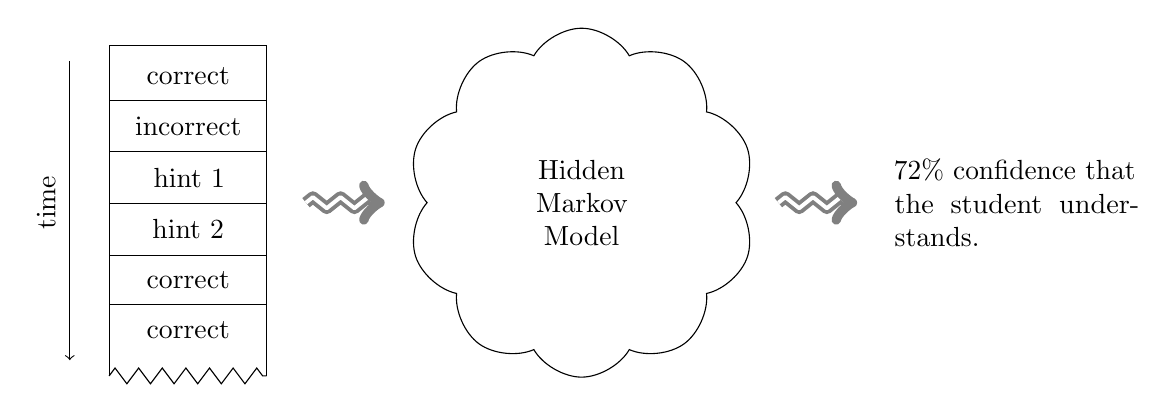
\begin{tikzpicture}

\draw (-1,2) -- (1,2);
\draw (-1,2) -- (-1,-2.2);
\draw (1,2) -- (1,-2.2);

\draw [->] (-1.5,1.8) -- (-1.5,-2);

\node at (-1.8,0) [rotate=90] {time};

\draw [decorate, decoration={zigzag,segment length = 3mm, amplitude = 1mm}]  (-1,-2.2) -- (1,-2.2);

\node at (0,0) {\begin{minipage}{2cm}\begin{center}correct\\[.2cm] \hrule \vspace{.2cm} incorrect\\[.2cm] \hrule \vspace{.2cm} hint 1\\[.2cm] \hrule \vspace{.2cm}  hint 2 \\[.2cm] \hrule  \vspace{.2cm} correct\\[.2cm] \hrule \vspace{.2cm} correct \end{center}\end{minipage}};

\draw [->,gray, line join=round,line width=.5mm,double, double distance=.5mm,
decorate, decoration={
    zigzag,
    segment length=10,
    amplitude=2,post=lineto,
    post length=2pt
}]  (1.5,0) -- (2.5,0);

\node at (5,0) [cloud,draw,cloud puffs=10,cloud puff arc=120, aspect=1] {\begin{minipage}{1in}\begin{center}Hidden \\ Markov\\ Model\end{center}\end{minipage}};

\draw [->,gray, line join=round,line width=.5mm,double, double distance=.5mm,
decorate, decoration={
    zigzag,
    segment length=10,
    amplitude=2,post=lineto,
    post length=2pt
}]  (7.5,0) -- (8.5,0);

\node at (10.5,0) {\begin{minipage}{1.2in}72\% confidence that the student understands.\end{minipage}};

\end{tikzpicture}
\end{center}
  \caption{Diagram of the MOOCulus hidden Markov model.}
\end{figure}

Once the MOOCulus data is collected, it is fed into a hidden Markov
model to produce an estimate of the student's
understanding. Essentially, the students are assumed to be in one of
two states: ``knowing'' and ``unknowing.''  From the students'
performance on the exercises provided by MOOCulus, the hidden Markov
model decides what state each student is in.  For example, the time series data
$$
\mbox{correct},\quad\mbox{incorrect},\quad\mbox{correct},\quad\mbox{incorrect},\quad\mbox{correct},\quad\mbox{incorrect}
$$
is not strong evidence that the student is in the hidden ``knowing''
state.  On the other hand, time series data which would,
superficially, result in the same ``score'' of ``half right, half wrong,'' such as
$$
\mbox{incorrect},\quad\mbox{incorrect},\quad\mbox{incorrect},\quad\mbox{correct},\quad\mbox{correct},\quad\mbox{correct}
$$
is strong evidence of that the student has reached the ``knowing''
state.  The order matters.

The student receives additional practice problems of the same sort
until it is estimated that their understanding reaches a threshold, at
which point the student is given a new type of exercise and the
process repeats.  The overall goal is to keep providing exercises that
are difficult enough to be fun and educational, but not so easy as to
become boring and repetitive.  In spite of the fact that many tens of
thousands of students used MOOCulus, each experienced a personalized
path through the material.  In short, MOOCulus promises to enable
MOOCs to be massive, but not mass-produced.

\subsection*{Personnel}

In addition to both building MOOCulus and running Calculus One, Fowler
and Snapp have experience using technology and analyzing its
effectiveness.

\paragraph*{Jim Fowler.} Fowler built the mobile phone
clicker used to measure student engagement for OSU's technology
enhanced calculus lectures, and Fowler's research training includes
high-dimensional data analysis from a topological perspective.

\paragraph*{Bart Snapp.} Having taught Calculus Remote at OSU (CROSU),
Snapp has also worked with OSU's Center for Enterprise Transformation
\& Innovation to build interactive textbooks for the iPad, with the
goal of measuring student engagement while reading the textbook.
Snapp is teaching two sections of calculus during Fall~2013 which will
be making heavy use of MOOCulus.

\paragraph*{David Lindberg.} A student in the masters of mathematical
sciences program specializing in mathematics education, Lindberg has
experience with data analysis and programming experience with R,
python, and ruby.  Lindberg is currently working with Snapp on his
Master's thesis, which will be examining results from the MOOCulus
data set and the adaptive learning platform that MOOCulus represents.

\section{Research questions}

\begin{figure}
\begin{center}
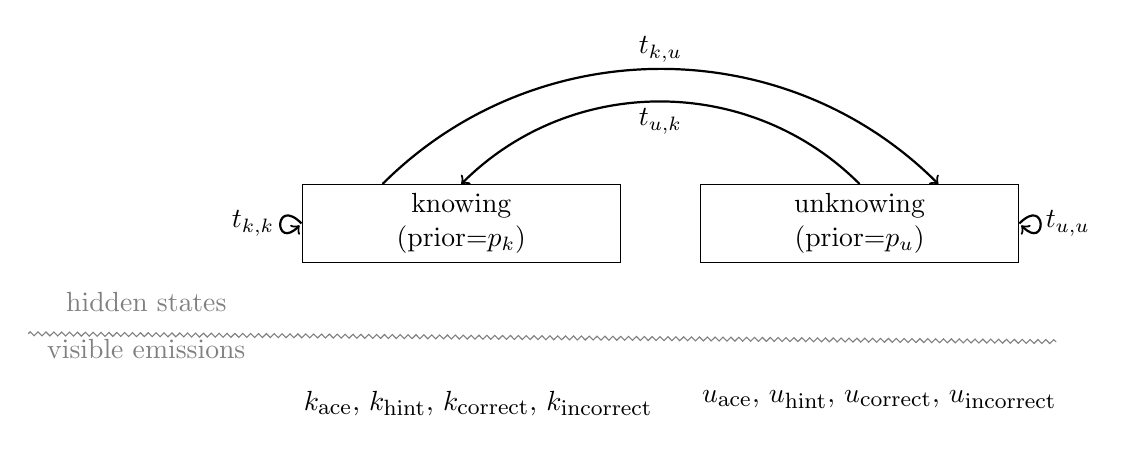
\begin{tikzpicture}
\tikzset{block/.style={rectangle,draw}}

  \node [block] (knowing) {\begin{minipage}{1.5in}\begin{center}knowing\\(prior=$p_k$)\end{center}\end{minipage}};
  \node [block, right=1 cm of knowing] (unknowing) {\begin{minipage}{1.5in}\begin{center}unknowing\\(prior=$p_u$)\end{center}\end{minipage}};

\path ([xshift=-1cm]knowing.north) edge[thick,->,out=45,in=135] node[align=center,yshift=0.25cm]{{$t_{k,u}$}} ([xshift=1cm]unknowing.north);
\path (unknowing.north) edge[thick,->,out=135,in=45] node [align=center,yshift=-0.25cm]{{$t_{u,k}$}}  (knowing.north);
\path ([yshift=0cm]unknowing.east) edge[thick,->,out=45,in=-45,loop] node [align=center,xshift=0.35cm]{{$t_{u,u}$}}  ([yshift=-0cm]unknowing.east);
\path ([yshift=0cm]knowing.west) edge[thick,->,out=135,in=-135,loop] node [align=center,xshift=-0.35cm]{{$t_{k,k}$}}  ([yshift=-0cm]knowing.west);

\node [xshift=0.5cm,below=1.5cm of knowing] (knowing-emit) {\begin{minipage}{5cm}$k_{\mbox{\footnotesize ace}}$, $k_{\mbox{\footnotesize hint}}$, $k_{\mbox{\footnotesize correct}}$, $k_{\mbox{\footnotesize incorrect}}$\end{minipage}};
\node [xshift=0.5cm,below=1.5cm of unknowing] (unknowing-emit) {\begin{minipage}{5cm}$u_{\mbox{\footnotesize ace}}$, $u_{\mbox{\footnotesize hint}}$, $u_{\mbox{\footnotesize correct}}$, $u_{\mbox{\footnotesize incorrect}}$\end{minipage}};

\draw [decorate, color=gray,decoration={zigzag,segment length = 1mm, amplitude = 0.25mm}]  ([xshift=-5.5cm,yshift=-0.9cm]knowing.south) -- ([xshift=2.5cm,yshift=-1cm]unknowing.south);

\node [color=gray,xshift=-4cm,below=0.25cm of knowing.south] (hiddens) {hidden states};
\node [color=gray,below=0.1cm of hiddens] (visibles) {visible emissions};

%\draw [decorate,decoration={brace,amplitude=10pt,mirror},yshift=0pt]
%([yshift=-1cm]knowing-emit) -- ([yshift=1cm]unknowing-emit) node [black,midway,xshift=2cm] {emissions};

\end{tikzpicture}
\end{center}
  \caption{Parameters in the HMM.}

  \label{fig:parameters}
\end{figure}

The hidden Markov model behind MOOCulus involves quite a few
parameters (see Figure~\ref{fig:parameters}).  A student is assumed to
be either ``knowing'' or ``unknowing'' with some prior probabilities
which must sum to one, meaning $p_k + p_u = 1$; as the student
explores an exercise, they may change states---perhaps developing new
misconceptions, or by unlearning prior misconceptions.  These
transition probabilities need to satisfy $t_{k,k} + t_{k,u} = t_{u,u}
+ t_{u,k} = 1$.  Whether knowing or unknowing, the student may submit
correct answers, incorrect answers, request hints: the emission
probabilities of doing so within each hidden state must likewise sum
to one, e.g.,$k_{\mbox{\footnotesize ace}} + k_{\mbox{\footnotesize
    hint}} + k_{\mbox{\footnotesize correct}} + k_{\mbox{\footnotesize
    incorrect}}=1$.  There are, therefore, nine free parameters for
each exercise to set by hand.

Choosing the appropriate values which yields an accurate model of
student understanding takes a great deal of instructor intervention
and skill \parencite{romero2010educational}; can this be automated?
Can those hand-chosen parameters be justified?

Student data provides a method for doing precisely this.  As students
interact with MOOCulus, the data needed to refine the parameters of
the hidden Markov model is obtained.  Specifically, under the proposed
activity, the Baum--Welch algorithm would be used to set those
parameters.

Many of the parameters are pedagogically meaningful.  To what degree
is a correct answer after three ``hints'' strong evidence of student
understanding?  What prior probability should be assigned to the
likelihood of a student to submit a correct answer on the first try?
The parameters depend strongly on the particular homework exercise;
some exercises are conceptually deep but procedurally easy, while some
questions are conceptually light but procedurally quite involved, so
even a strong student may make ``careless'' mistakes which the model
shouldn't count against him/her on those procedurally involved
exercises.  The hand-chosen parameters appear to work ``well enough''
in practice, but the analysis of the data is required to justify the
hand-chosen parameters, and refinement may improve the student
experience. This leads to three basic questions:
\begin{itemize}
\item What parameters in the adaptive learning model best align online
  student performance with in-class student performance?
\item To what extent does student use of adaptive learning correlate
  with success in traditional, in-person courses?
\item Should the proposed model of student performance (i.e., two
  categories) be refined into additional categories?  
\end{itemize}
The former question addresses improving the hidden Markov model that
powers MOOCulus; the second question gets deeper, by addressing the
extent to which adaptive learning helps with in-person courses.

These questions, though framed in the setting of a calculus class, are
actually quite general; discipline specific education research is
inherently interdisciplinary \cite{dber-report}.  The MOOCulus
platform has already been used in the aforementioned English writing
MOOC---the so-called WexMOOC \parencite{gates-foundation-grant}; there
has been interest from other departments on campus and from the Office
of Distance Education at OSU.  These research questions, and the
resulting improvements to an open-source adaptive learning platform,
would be of interest to both education researchers and educators
alike, regardless of their chhosen content area or specialty of
expertise.

\section{Data sources}

A large data set already exists from the first run of the Calculus One
MOOC in Spring 2013; with a total enrollment of 47k~students, the
course still had 11,000 students engaging with the material after four
weeks, and 2,000 students at Week~15.  Altogether, a total of
2,079,428 correct answers were submitted to MOOCulus, with a total of
10.3 person-years having been spent by students working problems.  The
activity logs are stored in a SQL database and this database is
imported for analysis into R.

A second iteration of the Calculus One MOOC has been started at OSU
for Fall 2013.  There are already 25k students enrolled in that second
run.  In addition, Snapp is teaching two on-campus calculus courses: a
course for engineers and a course for teachers.  Fowler and Snapp have
obtained a letter of final determination from the Institutional Review
Board facilitating the use of human subjects in our research.  The
proposed plan is to have each of these groups of students enroll in
MOOCulus so that we can directly compare students' performance in the
online course with their in-class performance.

\section{Methodology}

\paragraph{Hidden Markov parameters.}

The data will be analyzed in R.  The Baum--Welch algorithm will be used
to set the parameters in the hidden Markov model. This will allow the
parameters in the MOOCulus hidden Markov model to be set for each
problem separately.  These parameters are independently of interest to
researchers, and they also will provide for a better student
experience for MOOCulus in Spring 2014.

\paragraph{Correlation to success.}

To assess the correlation between success in the MOOC and success in
the traditional course, in addition to teaching the online MOOC, Snapp
is teaching calculus to two---quite different---student populations in
Fall 2013.  The first is a calculus course for middle school teachers
($n=28$). In this course, students will complete online assignments on
MOOCulus as part of their grade.  The second is a calculus course for
engineering students ($n\approx 200$).  In this course, students will
be encouraged to work online problems in MOOCulus, but there will be
no grade attached to their progress.  By involving his in-person
students also in the online MOOCulus course, the extent to which
participation in the adaptive learning system correlates with success
on in-person assessments can be determined.

\section{Budget needs}
A course buyout provides necessary time for Snapp to perform the data
analysis, to write up the results, and to oversee the analysis work of
his Master's student, Lindberg.  One course buyout for Snapp is 15\%
of the combination of his base salary (\$60132) plus 29.6\% in
benefits. For Spring 2013, this amounts to $.15 \cdot 1.296\cdot
60132=\$11690$.  To release Lindberg from his teaching further costs
\$1925/month plus 12.6\% in benefits; for the Spring Semester from
January--May, this costs $\$1925 \cdot 5 \cdot 1.126 = \$10838$.
Altogether, the total cost for the two researchers' time is \$22528.

% travel money to get to http://www.educationaldatamining.org/EDM2014/

\pagebreak
\printbibliography

\end{document}

%%% Local Variables: 
%%% mode: latex
%%% TeX-master: t
%%% End: 
